\documentclass[a4paper, 11pt]{article}

\usepackage[utf8]{inputenc}		% LaTeX, comprends les accents !
\usepackage[T1]{fontenc}      	% Police contenant les caractères français
\usepackage[french]{babel}  
\usepackage{float}
\usepackage{lscape}
\usepackage{pdflscape}
\usepackage{mdframed}
\usepackage{hyperref}
\usepackage{graphicx}  % pour inclure des images

\usepackage[a4paper,left=2cm,right=2cm, bottom=2.5cm, top=2.5cm]{geometry}% Format de la page, réduction des marges
\graphicspath{ {./images} }

\AddToHook{cmd/section/before}{\clearpage}
%\pagestyle{headings}         	% Pour mettre des entêtes avec les titres
                             	% des sections en haut de page

% Les paramètres du titre : titre, auteur, date
\title{Projet de programmation}
\author{Groupe \emph{08}\\
	\emph{Mateo Avventuriero, Livio Nortes-Bousquet, Hugo Vaillant et Donovann Zassot}\\
    L2 informatique\\
  Faculté des Sciences\\
Université de Montpellier.}
        


\begin{document}
\vspace*{1cm}
\centerline{\Huge\bf HAI405I}
\vspace*{1.5cm}
\begin{center}              	% pour centrer 
							


\includegraphics[width=8cm]{logo.png}   % insertion d'une image


\end{center}
\vspace*{1.5cm}

\begin{mdframed}
\centerline{\Huge Projet de programmation}
\end{mdframed}

\vspace*{1.5cm}

\noindent{\large\bf Groupe 08 :}

\begin{itemize}
\item Mateo Avventuriero
\item Livio Nortes-Bousquet
\item Hugo Vaillant
\item Donovann Zassot
\end{itemize}
\vspace*{1.5cm}

\begin{center}
  L2 informatique\\
  Faculté des Sciences\\
Université de Montpellier.
\end{center}

\section{Organisation}
Pour la réalisation du projet informatique, notre équipe a choisi d'adopter une méthode agile. Cette méthode nous a permis de progresser efficacement en planifiant les tâches de manière itérative. 
Chaque semaine, généralement lors de la séance de TD, nous avons tenu une réunion d'avancement. Cette réunion était divisée en deux parties, on discutait d'abord des tâches accomplies lors de la semaine passée puis des prochaines taches à réaliser. 
Notre chef de projet, Donovann, prenait ensuite en charge la planification et l'affectation des tâches à réaliser dans la semaine, en s'assurant que celles-ci étaient claires et bien définies.

\vspace{3mm}
\begin{figure}[H]
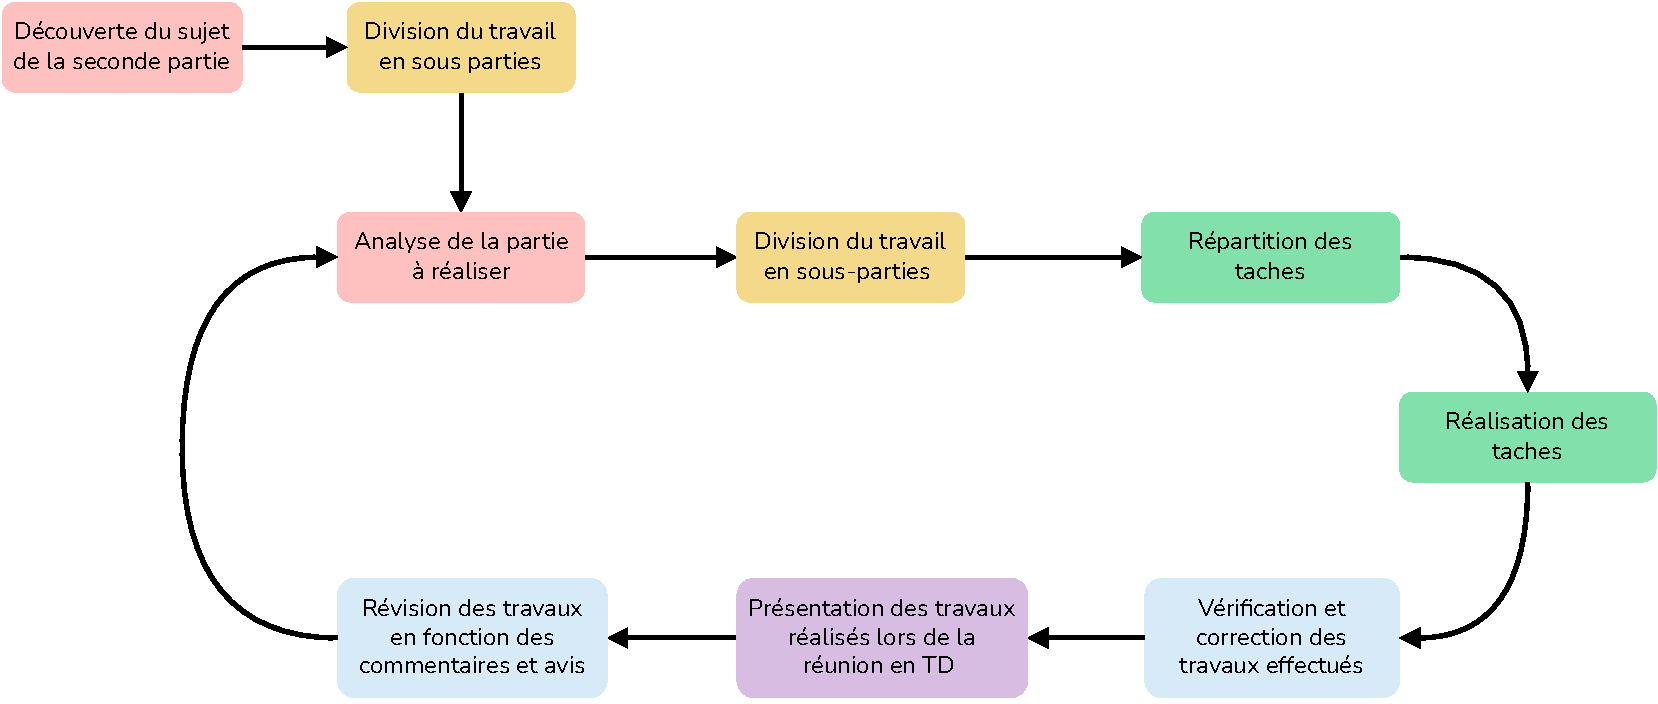
\includegraphics[width=\textwidth]{Organisation.pdf}
\caption{Diagramme des étapes de réalisation du projet}
\end{figure}
\vspace{2mm}

Afin de faciliter la collaboration au sein de l'équipe ainsi que le suivi du projet, nous avons utilisé plusieurs outils. Tout d'abord, nous avons choisi Github comme plateforme de gestion de versions pour stocker le code et suivre les modifications apportées par chaque membre de l'équipe au fil du temps. Cela nous a permis de collaborer plus efficacement et de garder une trace de l'évolution du projet.\\

Nous avons également utilisé un serveur Discord pour les communications inter-équipe, ce qui nous a permis d'organiser les discutions en différentes catégories (discussions techniques, questions, gestion du projet,...).\\

Dans l'ensemble, l'utilisation de ces outils nous a permis de travailler de manière plus efficace et d'améliorer la collaboration tout au long du projet. Les informations relatives à nos outils sont accessibles via les liens \href{https://github.com/}{Github}, \href{https://www.jetbrains.com/fr-fr/pycharm/}{PyCharm}, \href{https://www.jetbrains.com/fr-fr/webstorm/}{WebStorm} et \href{https://discord.com/}{Discord}.


\begin{landscape}
\begin{figure}[htbp]
\vspace{4mm}

  \centering
  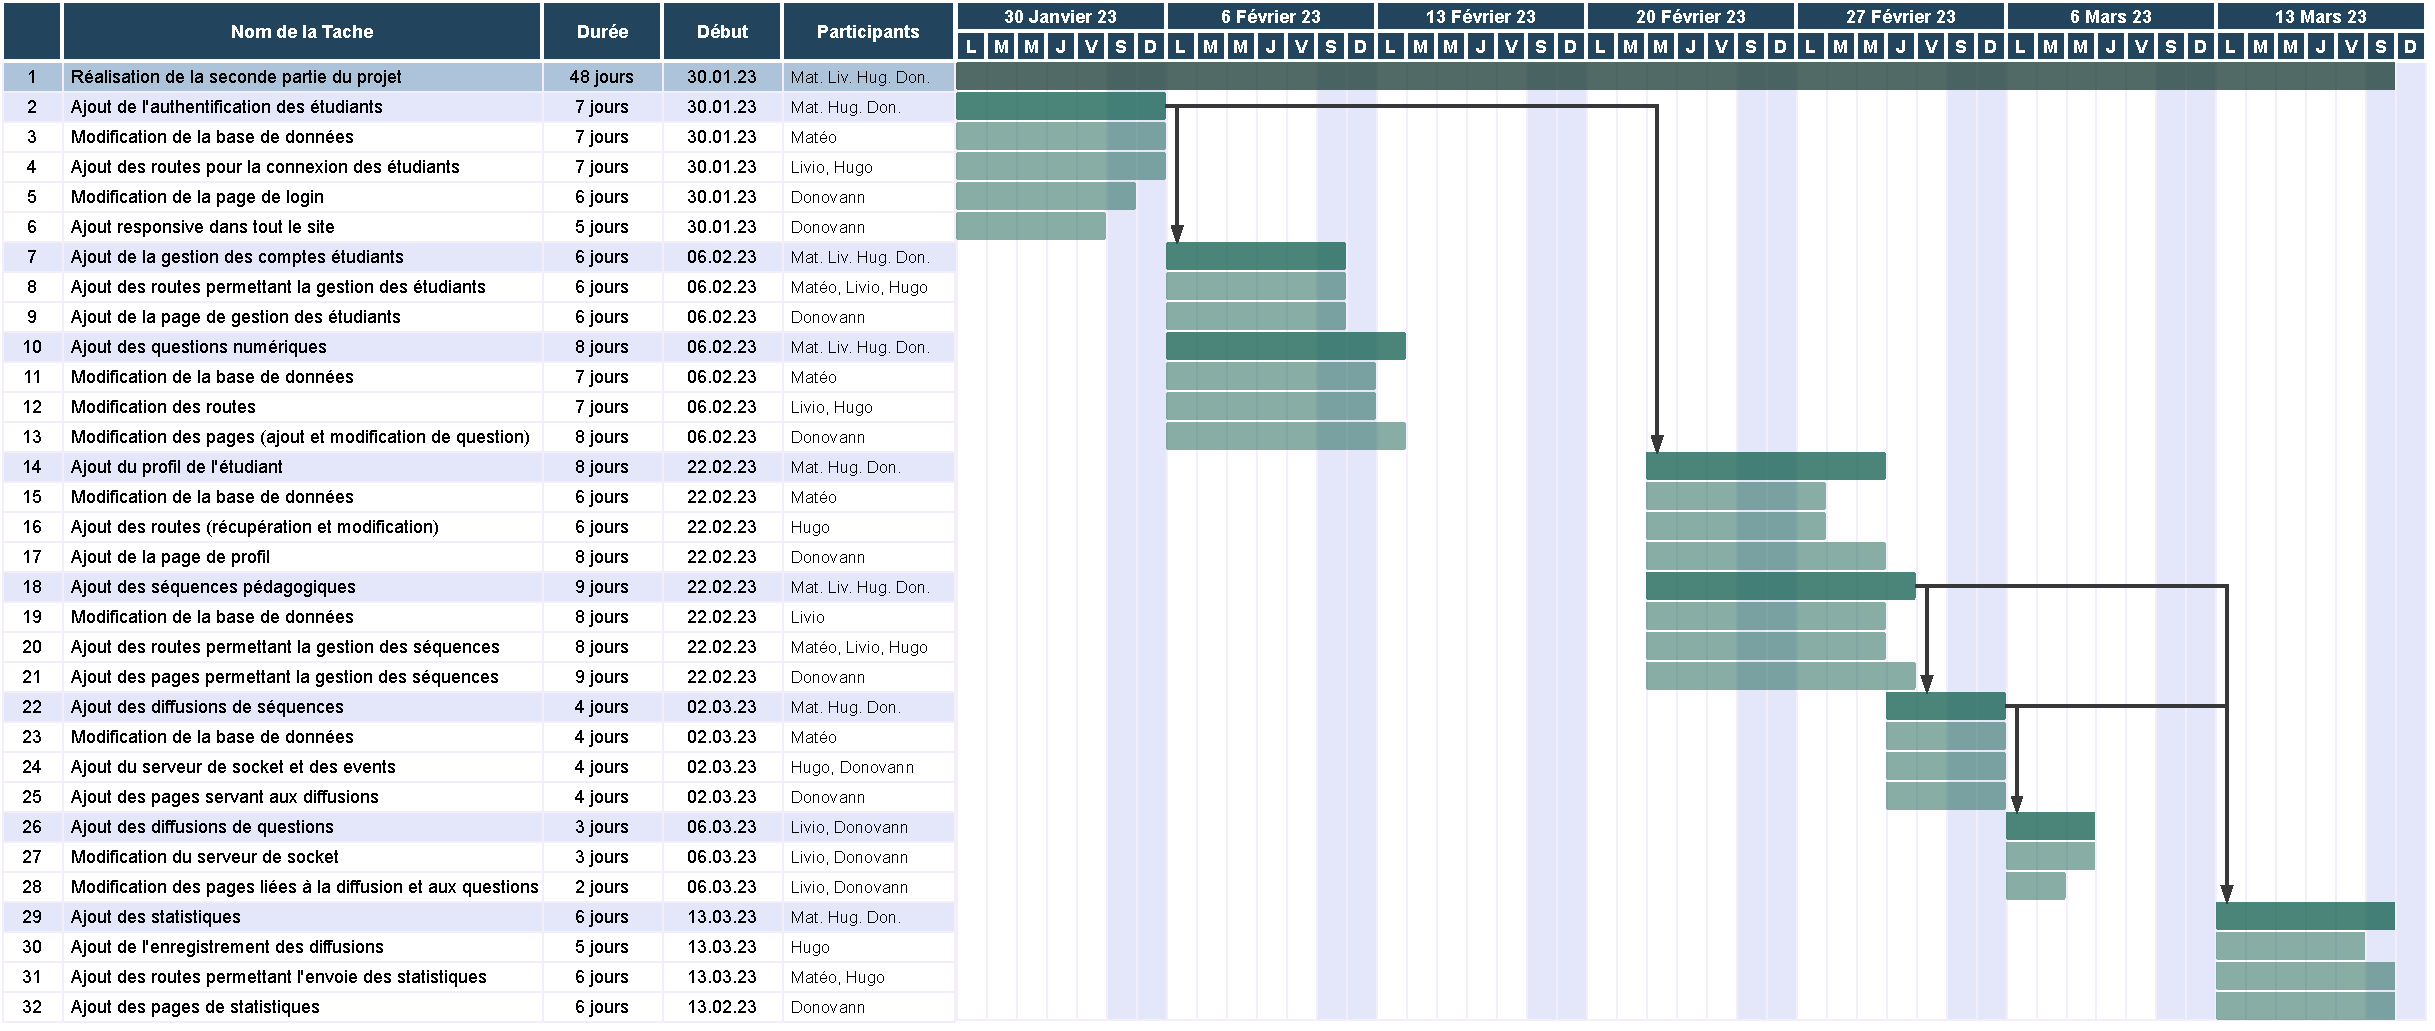
\includegraphics[width=\linewidth]{Gantt.pdf}
  \caption{Diagramme de Gantt du projet}
\label{fig:pdf-horizontal}
\end{figure}

Ce diagramme de Gantt est une représentation visuelle des étapes du projet. 
Les étapes du projet sont représentées par des barres horizontales. 
Chaque étape principale (vert foncé) peut comporter une ou plusieurs étapes secondaires (vert). 
Les flèches, quant à elles, indiquent les dépendances entre les étapes.\\\\

Il est important de noter que la réalisation de la vidéo présentant les fonctionnalités du site, ainsi que la rédaction du rapport, n'ont pas été prises en compte dans le diagramme de Gantt car elles ne faisaient pas partie intégrante du projet. Cependant, le projet a été planifié pour laisser suffisamment de temps pour la production de la vidéo ainsi que la rédaction du rapport.
\end{landscape}


\section{Cahier des charges}
Notre projet informatique intègre actuellement toutes les fonctionnalités prévues dans le cahier des charges. Nous avons donc atteint les objectifs fixés dans la présentation.\\

De plus, nous avons apporté des améliorations supplémentaires au projet par rapport au cahier des charges. Ces ajouts ont contribué à améliorer l'expérience utilisateur.\\

Nous avons, tout d'abord, amélioré la gestion des étudiants en permettant aux enseignant de supprimer les comptes des étudiants au cas par cas ou tous les étudiants en même temps, comme montré dans la figure \ref{fig:ajouts}.\\

Ensuite nous avons amélioré la gestion des étiquettes en permettant aux enseignants de modifier leurs étiquettes et de les supprimer comme le montre également la figure \ref{fig:ajouts}. Cet ajout permet d'offrir aux enseignants plus de flexibilité pour organiser leurs questions.\\

\vspace{2mm}
\begin{figure}[H]
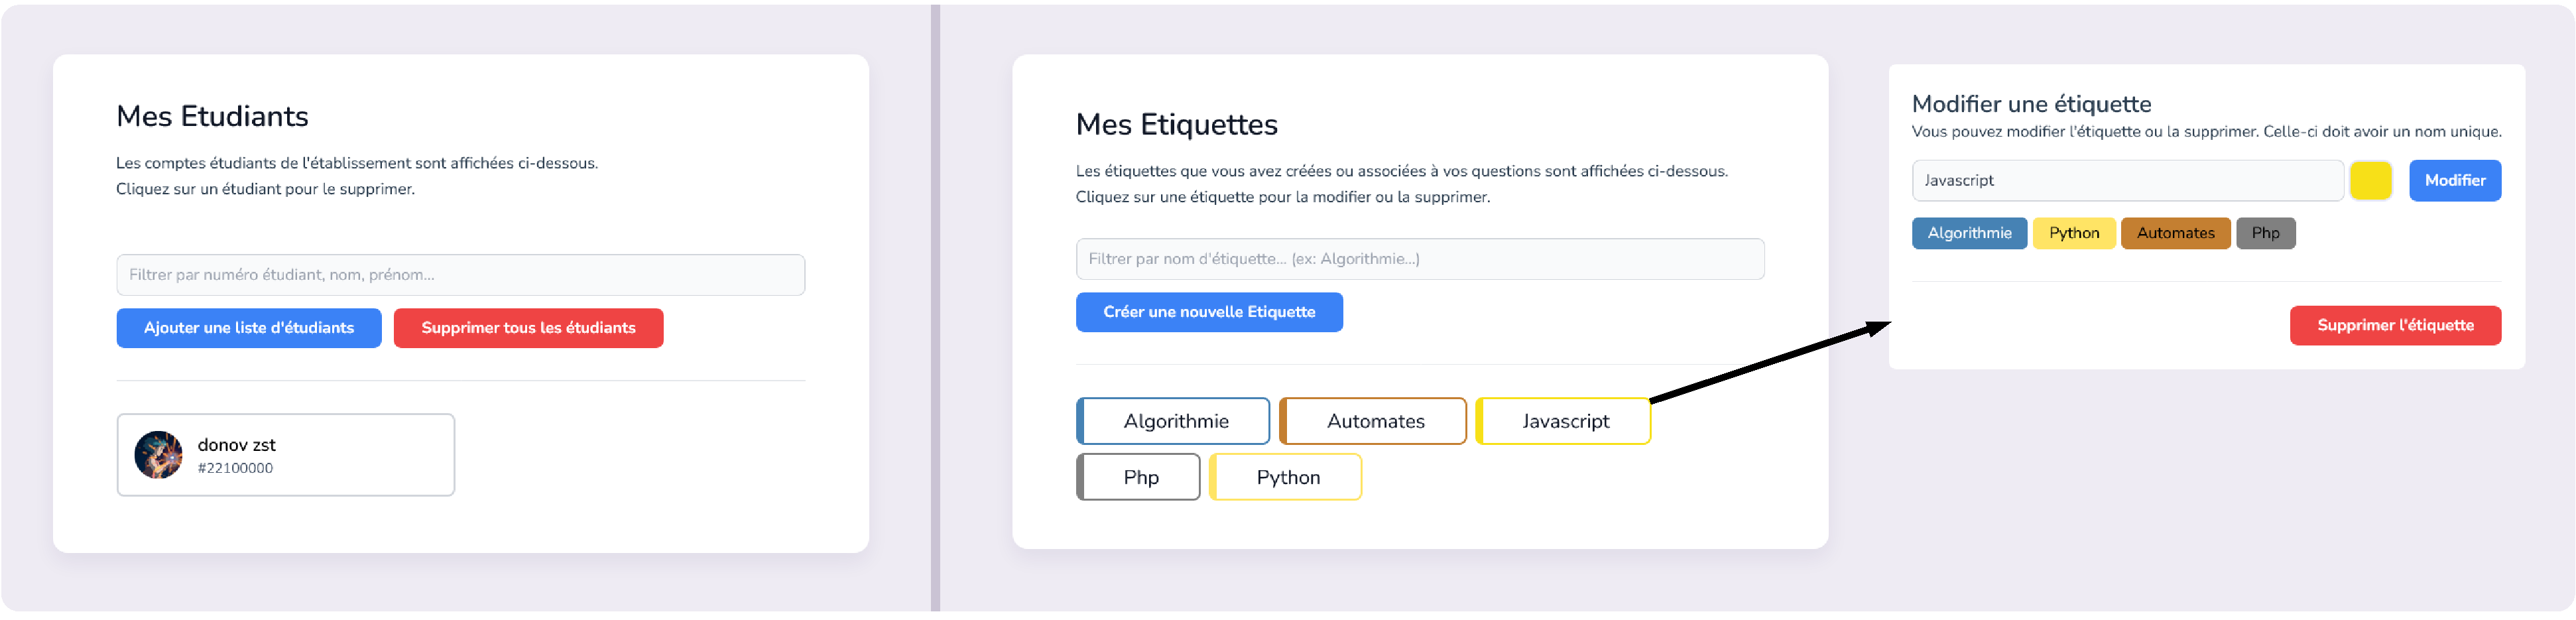
\includegraphics[width=\textwidth]{Ajouts.pdf}
\caption{Pages "Mes Etudiants" et "Mes étiquettes"}
\label{fig:ajouts}
\centering
\end{figure}
\vspace{3mm}

Nous avons aussi ajouté la possibilité, pour les étudiants, de personnaliser leur profil. Ils peuvent désormais modifier leur image de profil. Cette dernière est visible par les enseignants dans la page de gestion des utilisateurs et dans la page des statistiques. La couleur du profil, comme le montre la figure \ref{fig:profil}, est déterminée par la couleur prédominante de l'image de profil.\\

\vspace{2mm}
\begin{figure}[H]
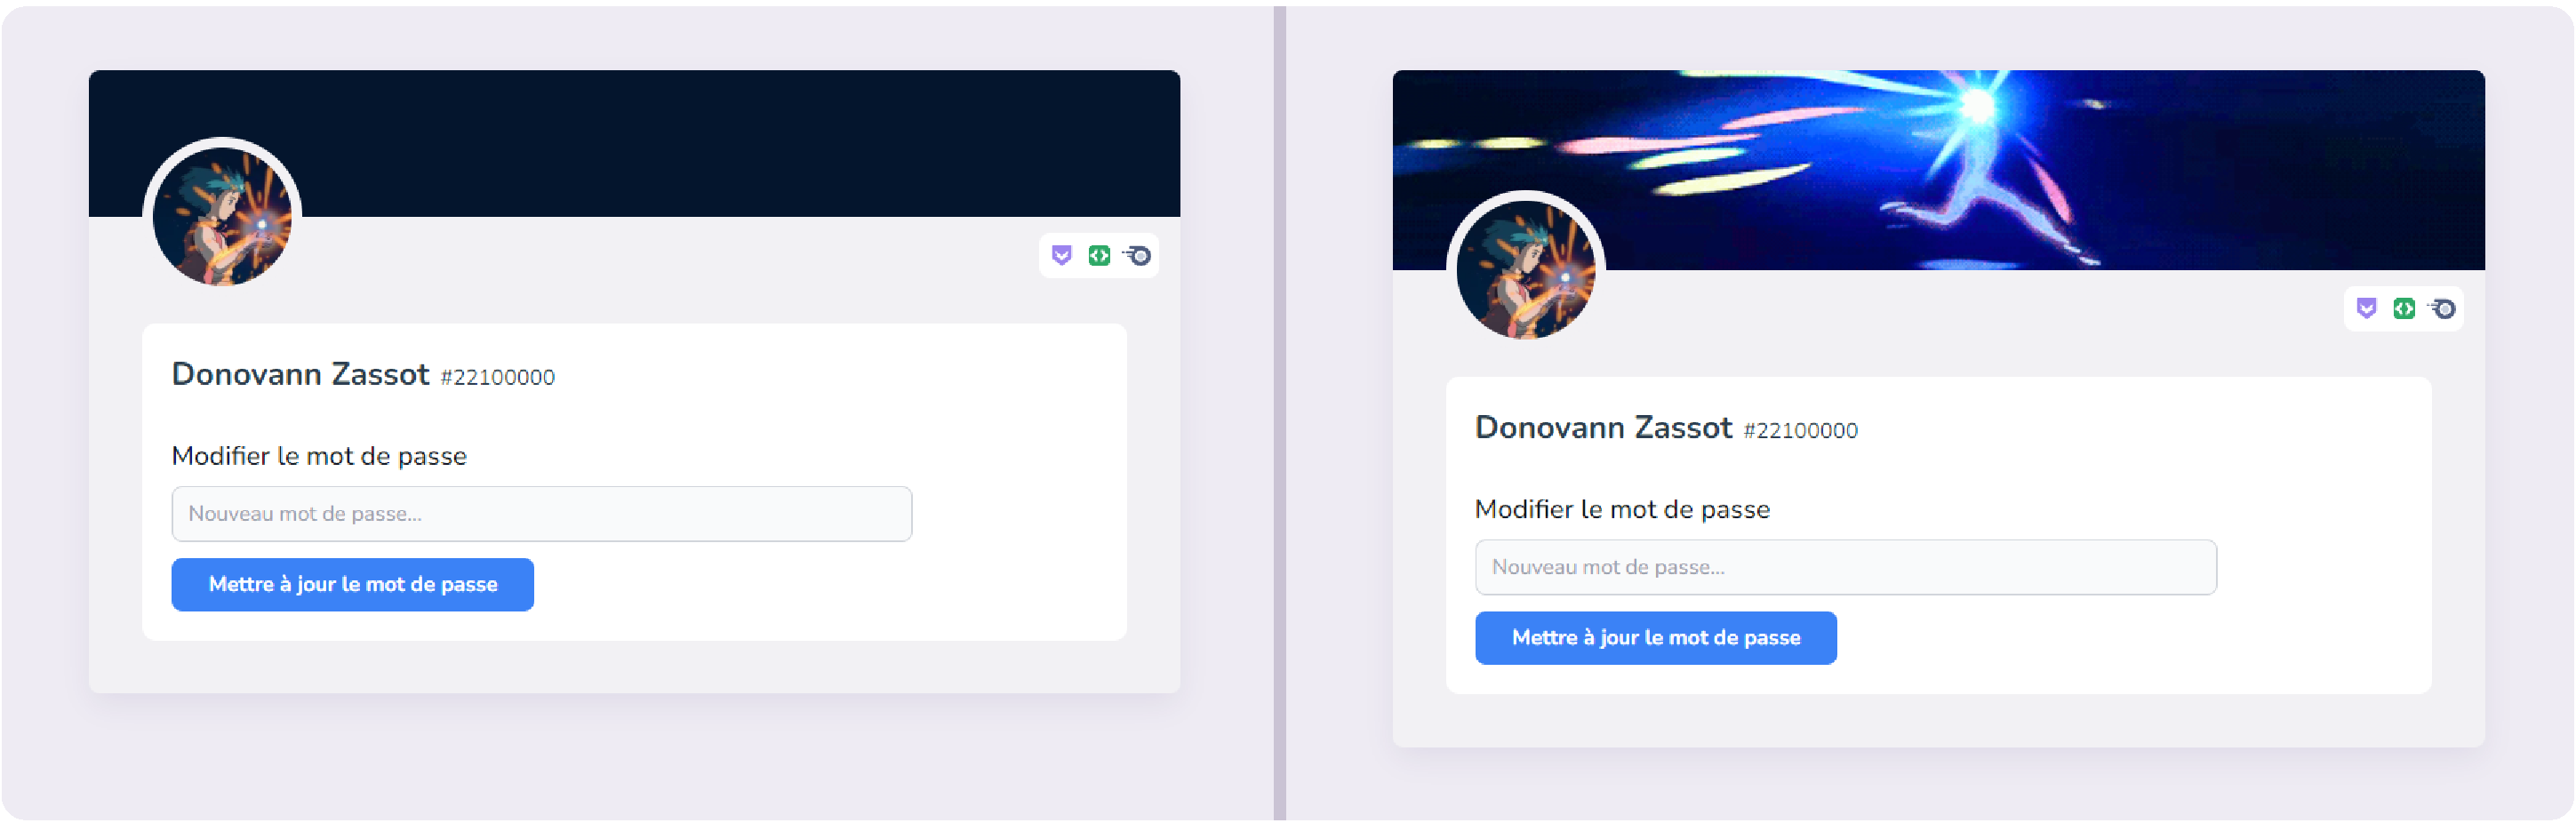
\includegraphics[width=\textwidth]{Profil.pdf}
\caption{Pages de Profil Etudiant (et la version de la page avec l'easter-egg activé)}
\label{fig:profil}
\centering
\end{figure}
\newpage

Enfin, pour rendre l'expérience utilisateur plus agréable, nous avons inclus plusieurs références et easter-eggs dans notre application. Parmi ceux-ci, vous trouverez :\\

\begin{itemize}
\setlength\itemsep{1em}
\item[•] La page de profil étudiant est une référence à l'interface utilisateur de Discord. En effet, nous avons, sur cette page uniquement, repris les éléments de design de Discord. Grâce à cela nous souhaitons créer une expérience familière pour les utilisateurs étudiants de notre site.

\item[•] Dans la page de profil étudiant, nous avons choisi les badges Discord. Le premier est une référence à la hypesquad de Discord avec le choix de la maison Bravery pour représenter l'équipe de développement\footnotemark[1], le second est le badge \textit{Developpeur Actif} et le troisième, le badge \textit{Nitro}.

\item[•] En cliquant sur un de ces badges, l'utilisateur débloque la possibilité de modifier le fond du profil étudiant comme avec Discord Nitro (côté client uniquement). Il peut alors choisir un fichier image qui sera défini comme fond. L'image peut être animée (gif). Vous pouvez avoir un aperçu du rendu dans la figure \ref{fig:ajouts}.

\item[•] La page d'accueil "Mes dernières Séquences" contient également un easter-egg. En cliquant sur le mot "champ", un carrousel apparaît. Celui-ci contient 5 images contenant des jeux de mots avec "champ". 

\item[•] Lorsqu'un étudiant rejoint une diffusion, il arrive sur une page d'attente. S'il le souhaite, il peut cliquer sur le mot "patience" pour jouer au Memory avec les mascottes du jeu (Bubule, Marinette ou Octave). Le jeu de mémory a été développé spécialement pour le projet, 7 listes de cartes sont disponibles et jouables aléatoirement. Le jeu montre aussi le nombre de tours joués et meilleur score qui est enregistré en local storage. La partie se termine automatiquement dès que la diffusion commence.
\end{itemize}

\vspace{3mm}
\begin{figure}[H]
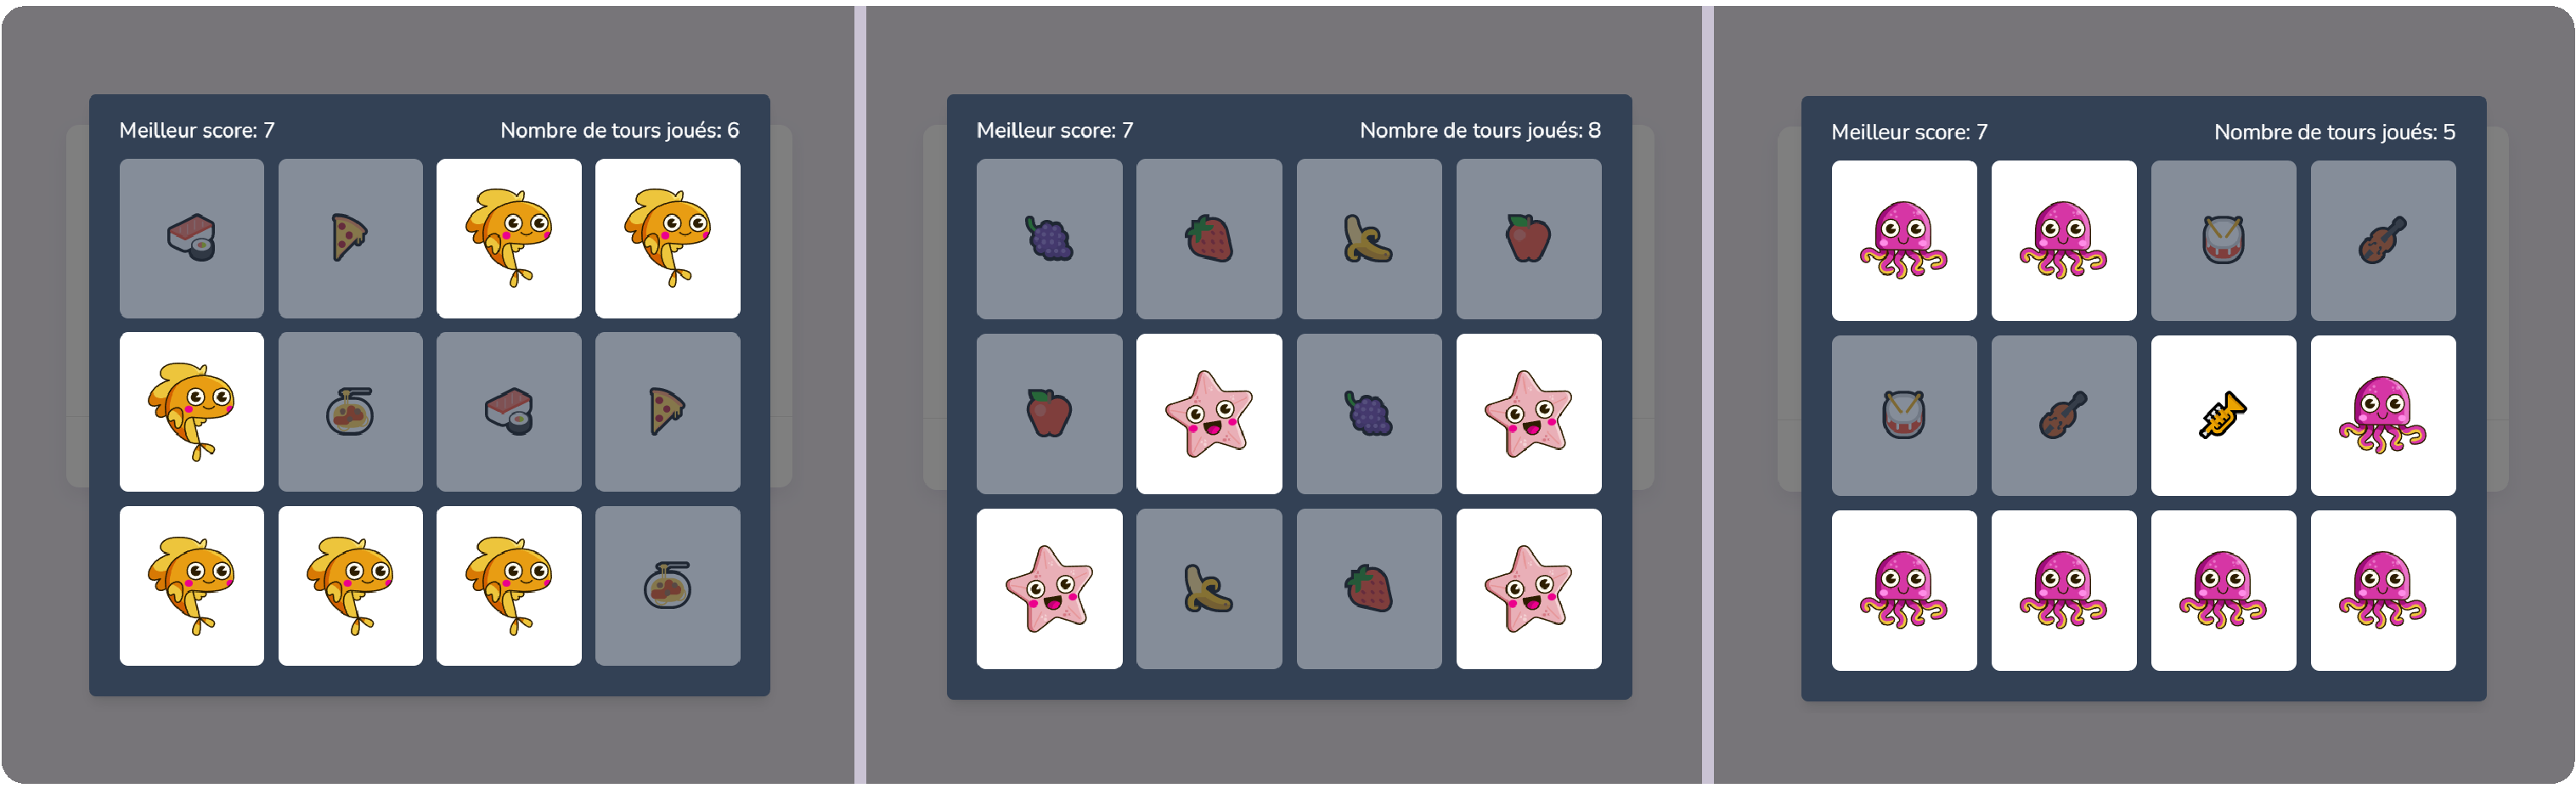
\includegraphics[width=\textwidth]{Memory.pdf}
\caption{Jeu de mémory avec les mascottes: un petit moment ludique !}
\label{fig:memory}
\centering
\end{figure}

\footnotetext[1]{Les quatre membres de l'équipe de développement font partie de la maison Bravery. Les maisons de la Hypesquad sont similaires aux maisons de Poudlard dans la série Harry Potter, où chaque maison représente une certaine qualité et des valeurs spécifiques. }

\section{Architecture et choix techniques}
\subsection{Architecture de l'application}
Notre application web est construite en deux parties distinctes pour séparer la logique de présentation de la logique métier.\\

La partie Front-End utilise Vue.js, un framework JavaScript progressif, pour créer une interface utilisateur intuitive et réactive. Le code est organisé en composants avec des fonctions spécifiques pour améliorer la lisibilité et la maintenance du code.\\

La partie Back-End utilise Flask, un framework Web minimaliste pour Python. Cette partie gère la logique métier et interagit avec la base de données SQLite. Le code, ici encore, est organisé en modules spécifiques pour faciliter la maintenance, en utilisant les blueprints de Flask. Cette approche modulaire permet également d'améliorer la lisibilité et la maintenance du code.\\

La communication entre les deux parties se fait via des appels HTTP pour récupérer, créer, modifier et supprimer des données. Nous avons également utilisé les sockets de Socket.io pour permettre une communication en temps réel entre les deux parties, notamment pour les diffusions des séquences.

\vspace{5mm}
\begin{figure}[H]
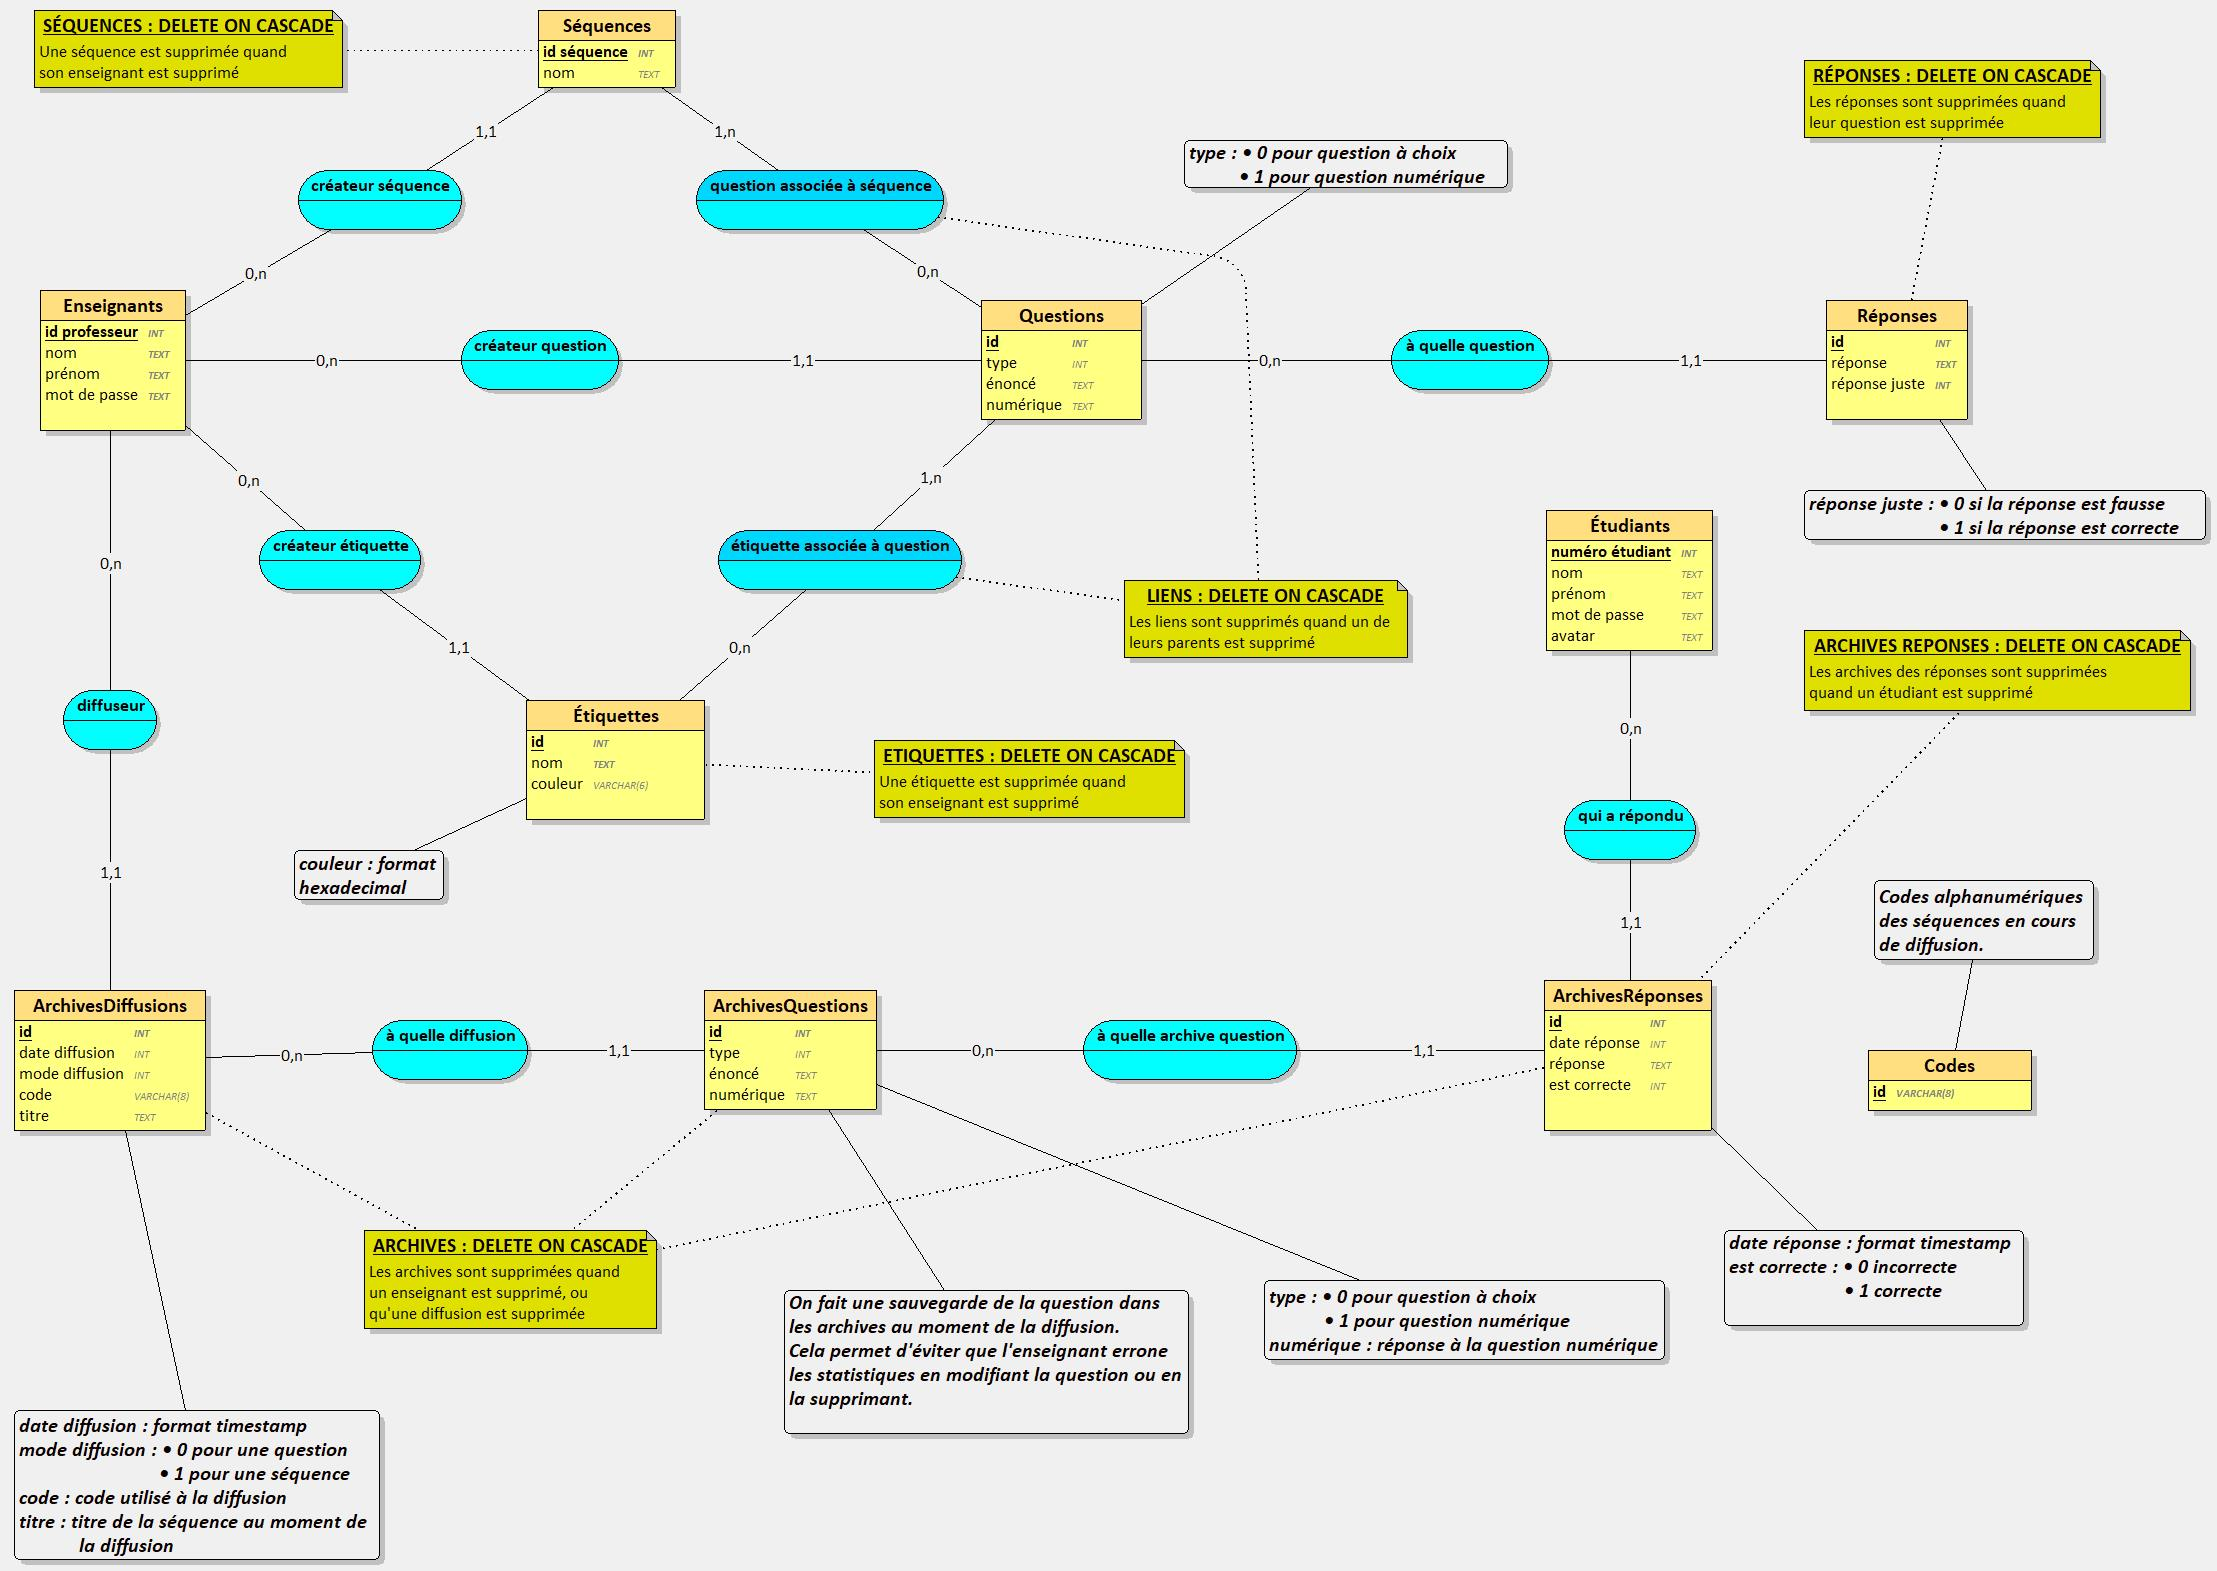
\includegraphics[width=\textwidth]{SchemaBDD.jpg}
\caption{Schéma de la base de données SQLite}
\end{figure}
\vspace{2mm}

\subsection{Choix techniques}
Le choix des technologies pour le développement d'un projet est crucial pour sa réussite. Dans cette partie, nous expliquerons les choix que nous avons faits pour notre application web.

\vspace{2mm}
\subsubsection{Flask : une architecture à base d'API}
Le choix d'utiliser Flask en tant que framework pour notre projet a été imposé par les contraintes du projet. Cependant, nous avons décidé de limiter son utilisation au strict minimum en ne l'utilisant que comme une API. Cette architecture présente de nombreux avantages, tels que la clarté de la séparation entre la logique métier et la présentation, comme mentionné précédemment. Cette séparation facilite grandement le développement en équipe et la maintenance des deux parties de manière indépendante, ce qui rend également l'application plus évolutive. Dans notre cas, où les différentes parties du projet sont découvertes au fur et à mesure, cette évolutivité est essentielle. 

\vspace{2mm}
\subsubsection{Base de données SQLite : avantages par rapport aux fichiers textes}
Nous avons soigneusement étudié plusieurs options de stockage de données, en évaluant leurs avantages et inconvénients respectifs. Après une analyse approfondie, nous avons décidé d'adopter une base de données SQLite.\\

L'utilisation d'une base de données présente de nombreux avantages, notamment une gestion efficace des données et une manipulation aisée. De plus, elle permet une structuration logique et cohérente des données, garantissant ainsi leur intégrité et évitant les erreurs de manipulation.\\

Outre les avantages précités, ce choix nous a permis de mettre en pratique les connaissances acquises lors du troisième semestre.

\vspace{2mm}
\subsubsection{Vue.js : un framework rapide et réactif}
Pour le développement de la partie Front-End de notre application, nous avons opté pour Vue.js. Et ce pour plusieurs raisons;
Nous avons tout d'abord été séduits par la rapidité du framework ainsi que sa réactivité. Ces deux avantages nous ont permis de créer rapidement une interface utilisateur intuitive et réactive.\\

Un autre avantage de Vue.js est sa facilité d'utilisation, en particulier pour les membres de l'équipe qui n'avaient pas d'expérience préalable avec des frameworks JavaScript. C'est Donovann qui a proposé Vue.js en raison de ses connaissances solides en React et de son désir de découvrir un nouveau framework.\\

Enfin, l'utilisation de Vue.js avec Flask nous a permis d'optimiser la vitesse de l'application, ce qui est un avantage considérable pour une application Web.

\section{Détail}
\subsection{Fonctionnement de la diffusion de quiz avec WebSocket}

\vspace{3mm}
\begin{figure}[H]
\centering
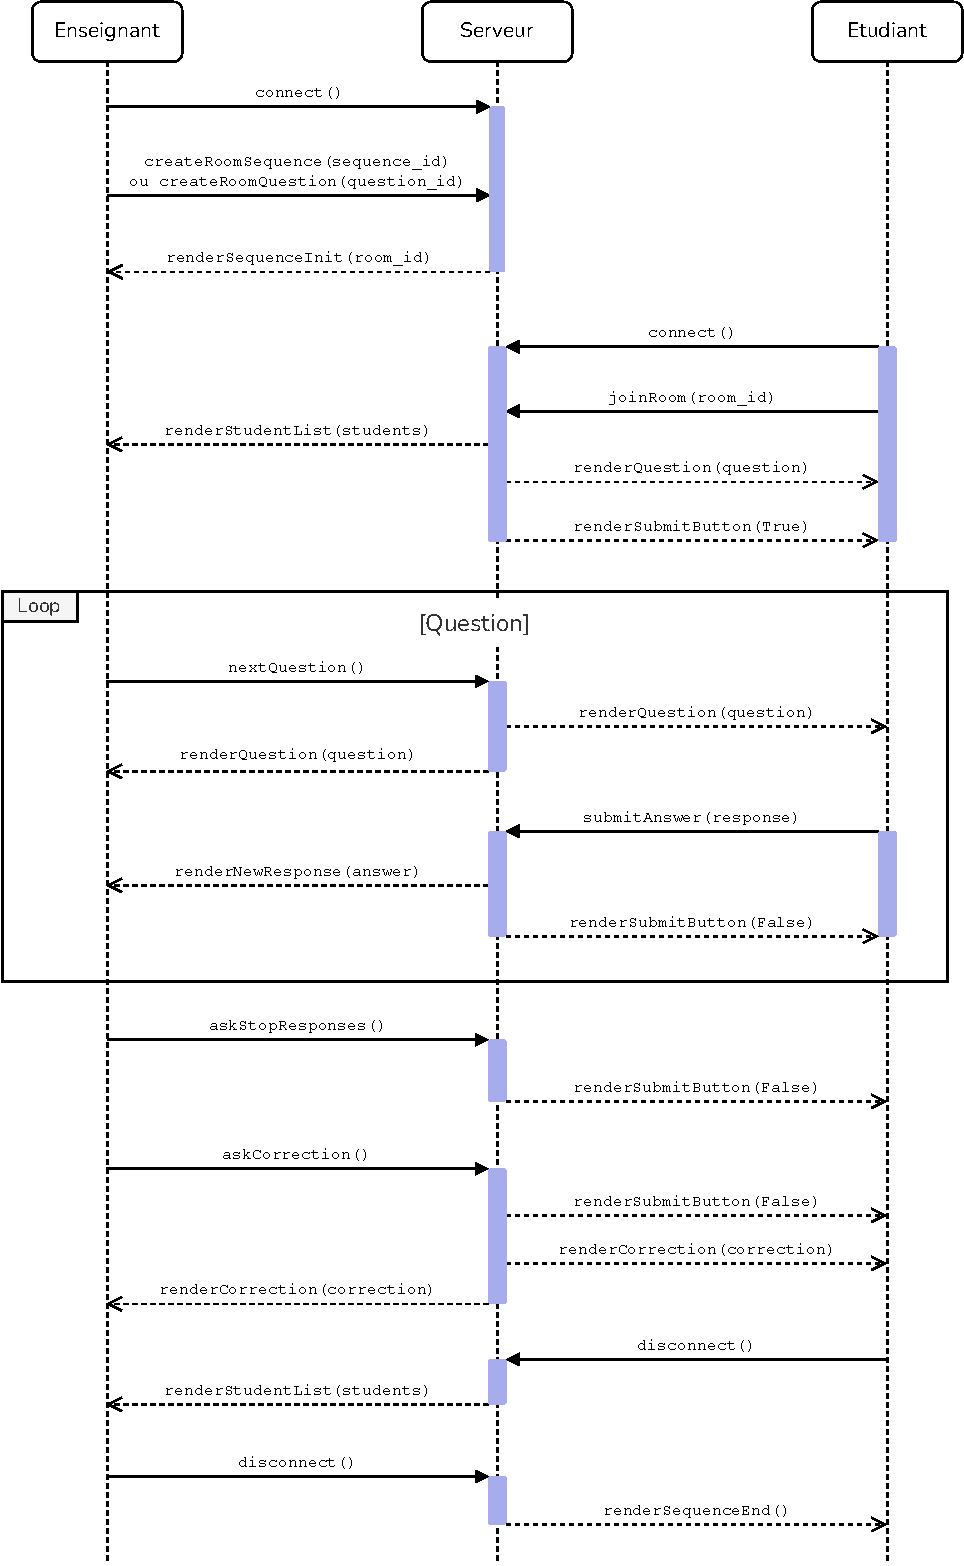
\includegraphics[width=13cm]{Diffusions.pdf}
\caption{Diagramme de séquence de la diffusion de quiz en direct avec WebSocket}
\label{fig:diffusions}
\end{figure}
\vspace{2mm}

Le diagramme de séquence présent dans la figure \ref{fig:diffusions} présente le diagramme de séquence qui décrit le fonctionnement des diffusions en direct sur notre site web. Ces diffusions utilisent un socket pour la communication en temps réel entre les enseignants et les étudiants.\\

Les enseignants peuvent créer une diffusion en émettant l'événement \texttt{createRoomSequence} ou \texttt{createRoomQuestion} en fonction du type de la diffusion. Cet événement déclenche la création d'une room Socket.IO et l'ajout de l'enseignant à cette dernière.\\

Les étudiants peuvent ensuite rejoindre la diffusion en entrant le code de la séquence, ce qui met à jour l'interface de l'enseignant en émettant l'événement \texttt{renderStudentList} à la room.\\

Les enseignants peuvent passer à la question suivante en émettant l'événement \texttt{nextQuestion} et les étudiants peuvent soumettre leur réponse avec \texttt{submitAnswer}. Les enseignants peuvent arrêter les réponses en émettant l'événement \texttt{askStopResponses} et demander la correction avec \texttt{askCorrection}.\\

Il est à noter que les enseignants ne sont pas obligés d'utiliser ces événements pour avancer dans la séquence et peuvent les utiliser dans l'ordre souhaité.

\vspace{5mm}
\subsection{Affichage des réponses en direct}
L'affichage des réponses en direct dans l'application est géré par une combinaison de deux composants : \texttt{StartSequenceView} et \texttt{RenderQuestion}.
Le composant \texttt{StartSequenceView} est le composant principal et est responsable de la gestion de la logique d'affichage des questions et des réponses en temps réel. 
Il utilise les composants \texttt{MultipleResponses} et \texttt{NumericResponses} pour afficher les réponses sous forme de graphique.\\

Les composant \texttt{NumericResponses} et \texttt{MultipleResponses} sont appelés en fonction du type de la question. Dans les deux cas les réponses numériques des étudiants sont affichées sur un graphique à barres, avec l'axe y représentant le nombre d'étudiants ayant donné une réponse spécifique, et l'axe x représentant les différentes réponses possibles. Le graphique est mis à jour en temps réel à mesure que les étudiants envoient leurs réponses. Comme demandé dans le cahier des charges, le site affiche maximum 5 barres (les 4 réponses les plus répondues et "Autres réponses").

\vspace{3mm}
\begin{figure}[H]
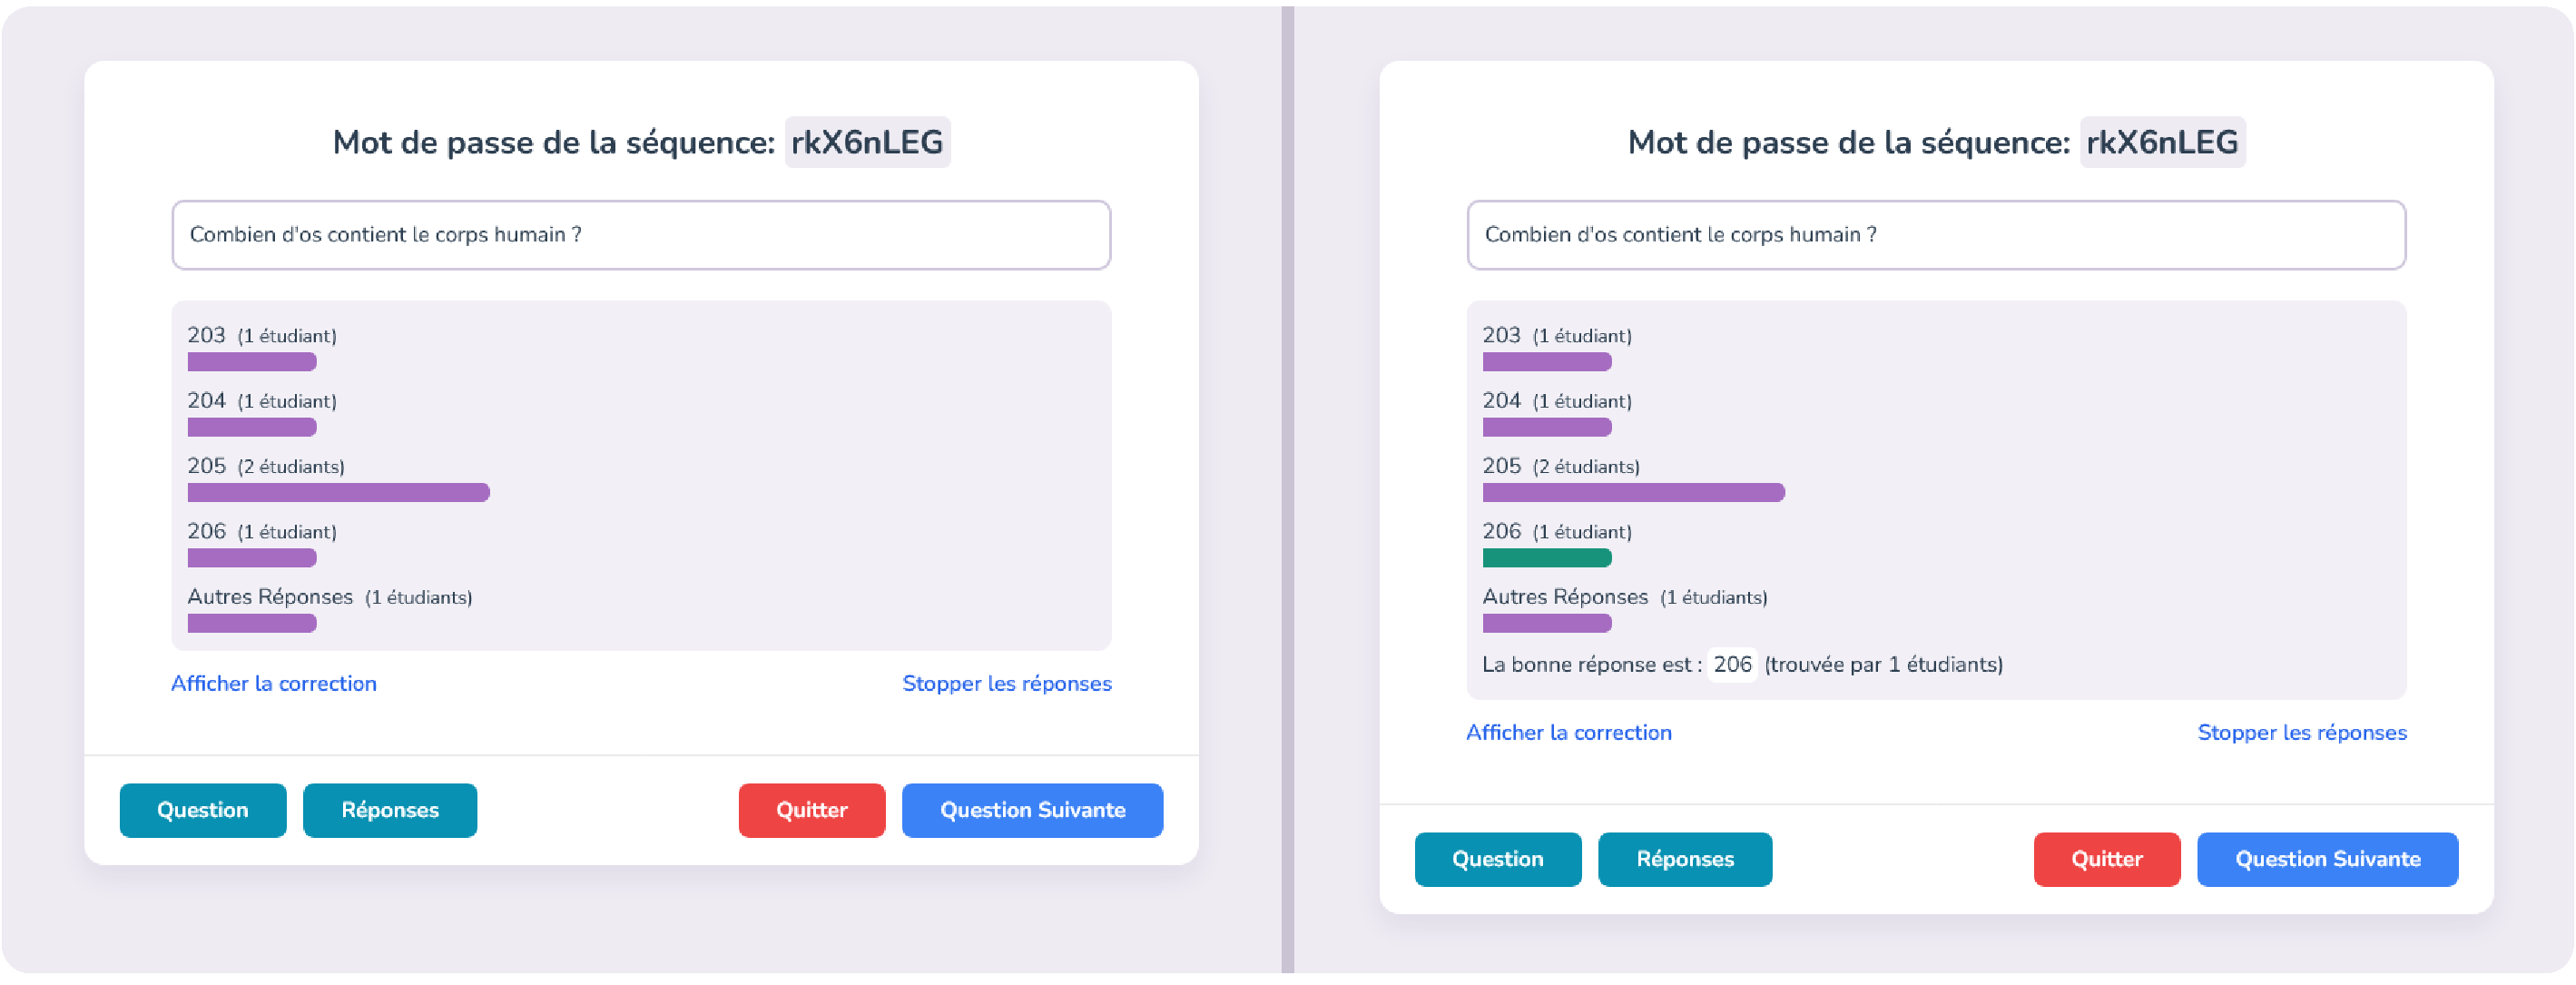
\includegraphics[width=\textwidth]{GraphiqueDiffusions.pdf}
\caption{Affichage des réponses en direct pendant la diffusion}
\end{figure}
\vspace{2mm}

\subsection{Authentification}
\begin{figure}[H]
\centering
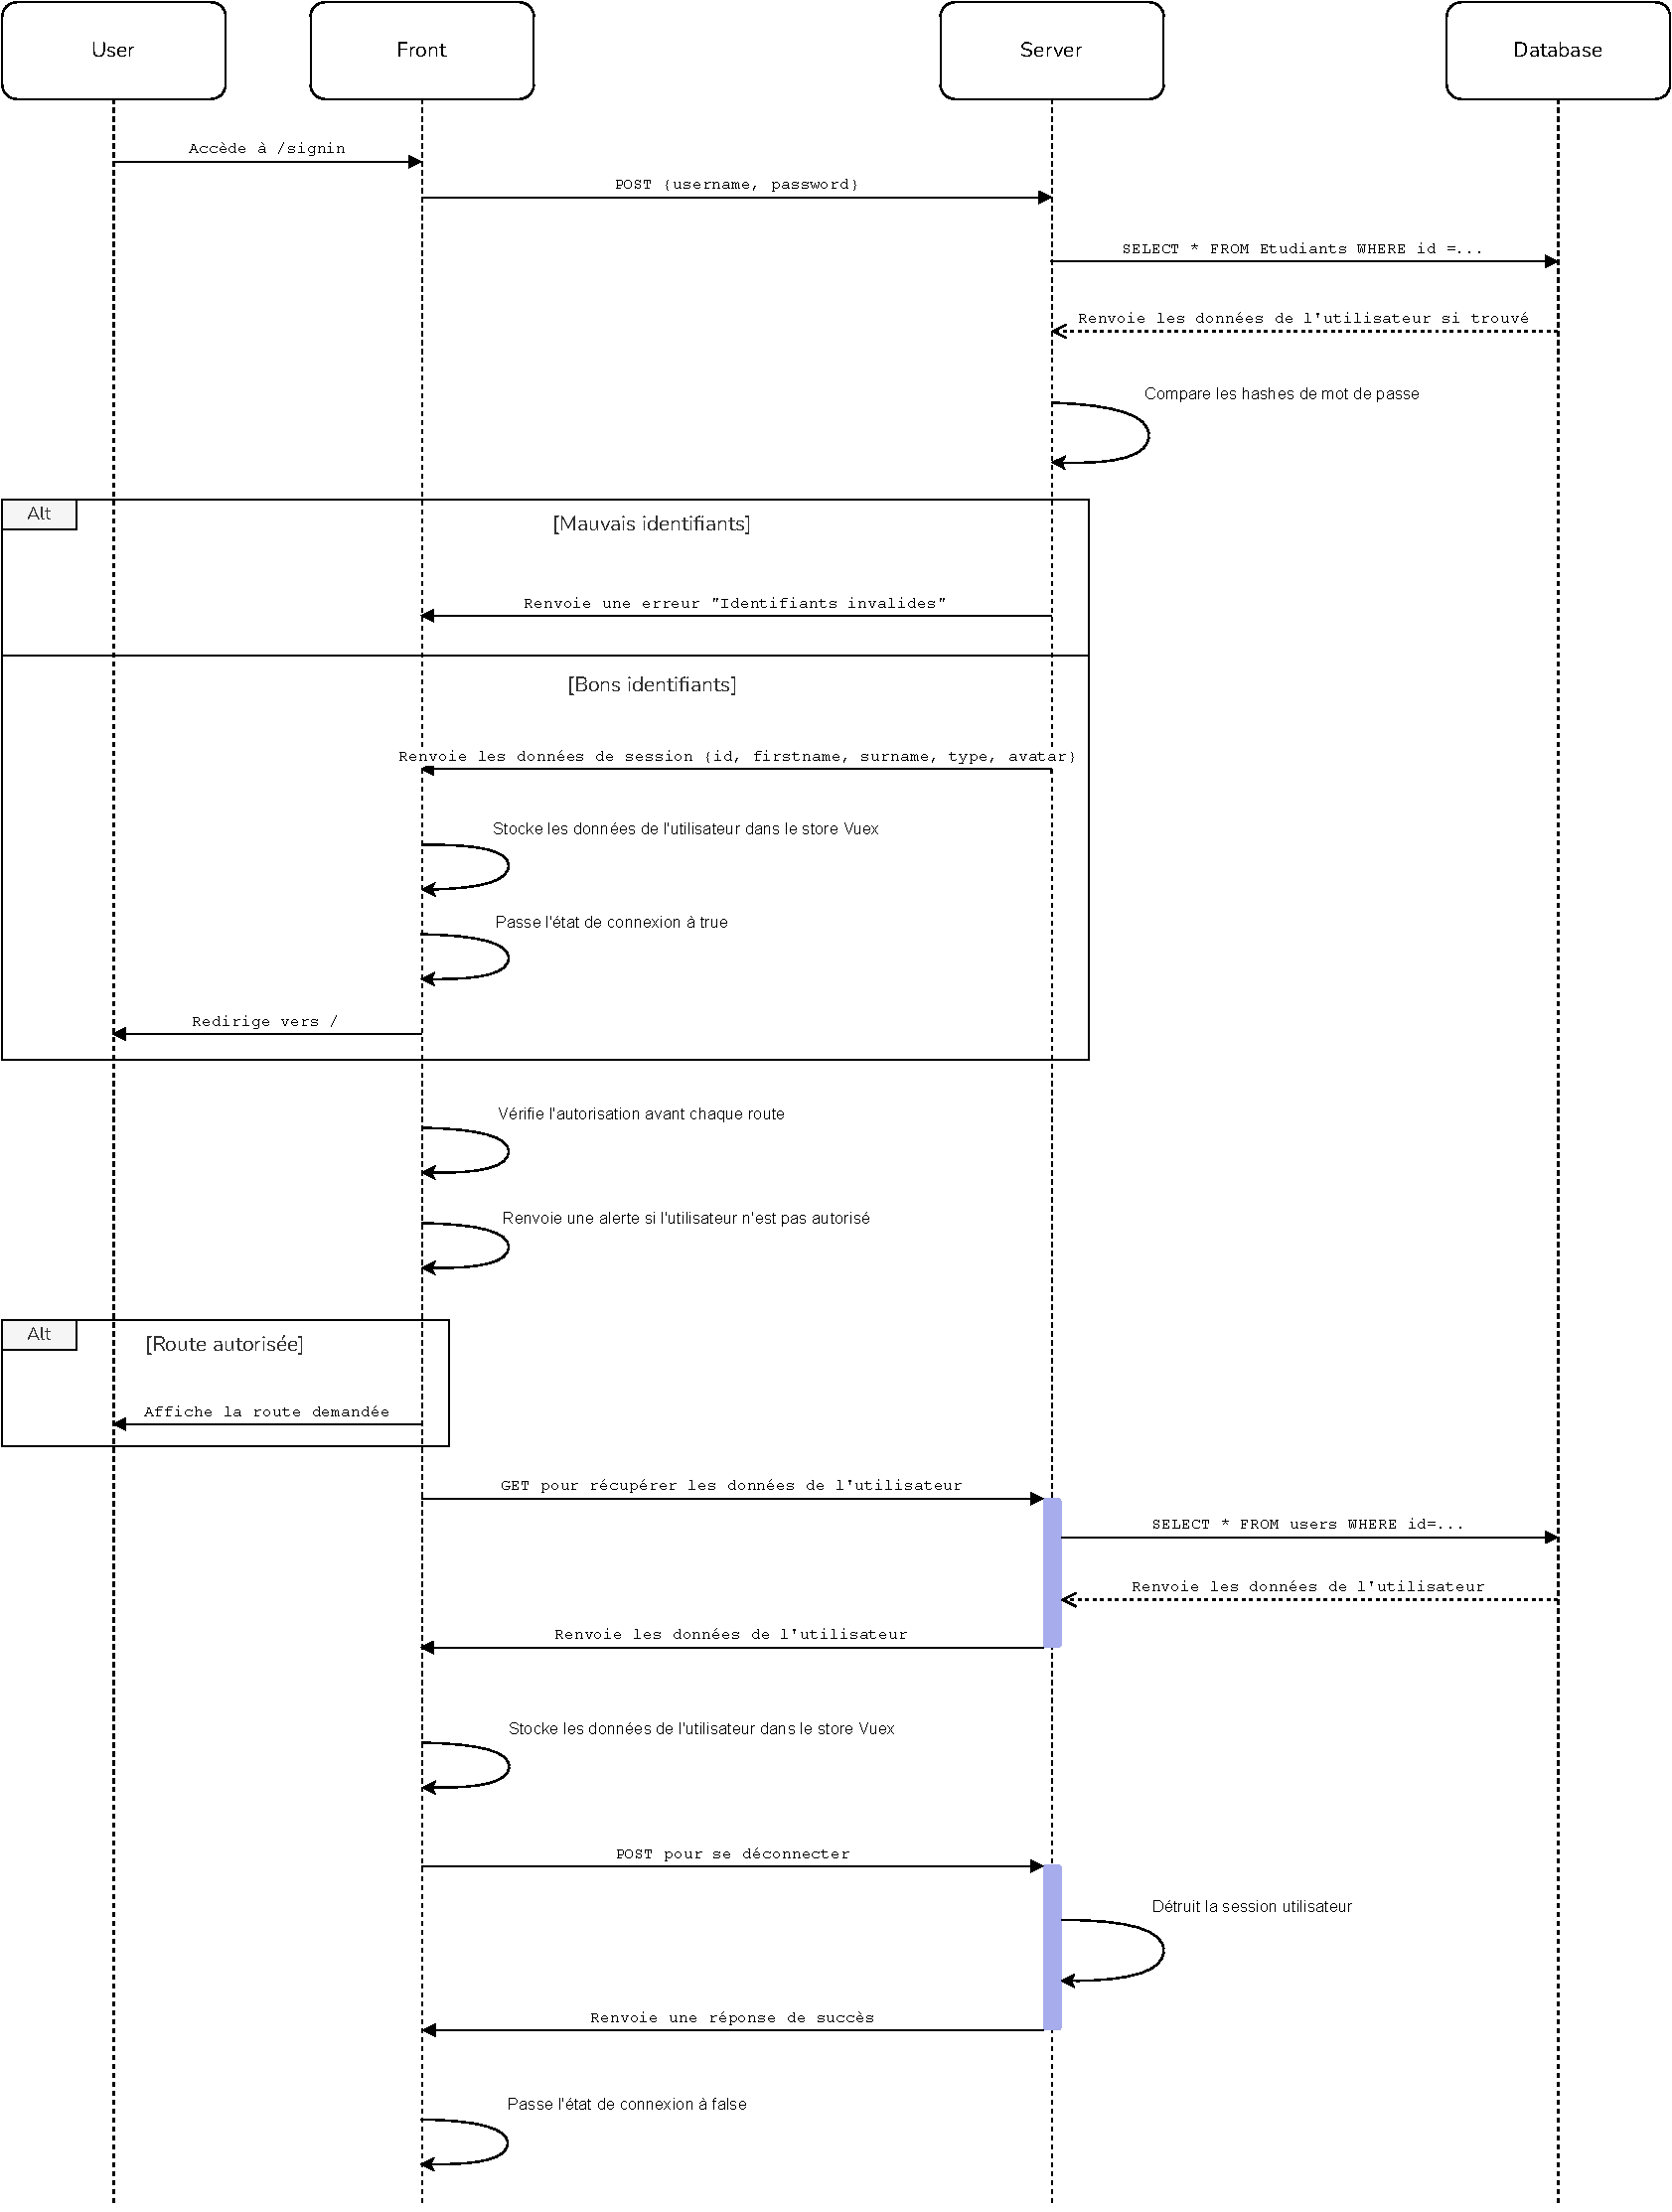
\includegraphics[width=\textwidth]{Authentification.pdf}
\caption{Diagramme de séquence pour l'authentification des étudiants}
\end{figure}

Le diagramme de séquence illustre le processus d'authentification pour les étudiants. Tout d'abord, l'étudiant entre ses identifiants sur la page de connexion. Ces informations sont alors envoyées au serveur pour vérification. Si les identifiants sont corrects, le serveur renvoie une réponse positive à l'étudiant, qui est alors redirigé vers la page d'accueil de l'application.\\

Pendant ce processus, le client (l'étudiant) interagit avec le serveur à travers des requêtes HTTP pour communiquer les informations nécessaires à l'authentification. Le serveur, quant à lui, vérifie les informations et répond avec un message indiquant si l'authentification a réussi ou échoué. Si l'authentification est réussie, le serveur envoie également les informations sur l'étudiant qui sont stockées dans la base de données.\\

De plus, le diagramme montre l'utilisation de deux technologies pour gérer l'état de l'application: le store Vuex et le routage. Le store Vuex permet de stocker les informations de l'utilisateur et de les rendre disponibles dans toute l'application. Le routage permet quant à lui de gérer la navigation entre les différentes pages de l'application et de vérifier si l'utilisateur est authentifié avant de lui donner accès à certaines pages.\\

En somme, ce diagramme de séquence représente de manière détaillée le processus d'authentification pour les étudiants dans l'application, tout en montrant les technologies utilisées pour gérer l'état de l'application.


\section{Bilan}
Notre projet de programmation Quizzly nous a permis d'appliquer de nombreuses connaissances acquises à la fac, telles que la gestion de bases de données, la programmation web avec les sockets et l'utilisation de schémas découverts en modélisation de niveau 2 pour la rédaction de ce rapport. Nous avons été ravis de pouvoir mettre en pratique ces compétences et de voir comment elles pouvaient être appliquées dans un projet concret.\\

Lors la première partie du projet, nous avons pris des décisions judicieuses qui se sont avérées scalables et qui ont permis de gagner du temps et des efforts pendant la deuxième partie du projet. Par exemple, nous avons choisi d'utiliser une base de données au lieu de fichiers textes, contrairement à ce que suggérait la présentation. Ce choix nous a permis de gérer les données plus facilement et d'effectuer des opérations plus complexes sur ces données. Nous pouvons prendre pour exemple ici les requêtes effectuées pour la partie statistiques du site.\\

Cependant, cette deuxième partie du projet nous a donné plusieurs défis.
Il fallait d'une part gérer la coordination des membres de l'équipe et faire attention au respect des délais, mais aussi de l'autre part, anticiper les contrôles continus et les devoirs demandés par la fac. 
Cette tâche n'était pas facile, car elle exigeait de planifier le travail à long terme tout en respectant les délais à court terme. 
Malgré cela, nous avons réussi à définir les priorités et les échéances pour chaque tâche, ce qui nous a permis de livrer un projet fonctionnel et de qualité dans les délais impartis.\\

En fin de compte, notre expérience sur Quizzly nous a appris beaucoup de choses sur la façon de travailler en équipe pour créer une application complexe. Nous avons découvert ce qui fonctionnait bien pour nous, et nous avons identifié des domaines dans lesquels nous pourrions nous améliorer pour devenir encore plus efficaces à l'avenir.

\end{document}